\documentclass[Ex4_Zusammenfassung.tex]{subfiles}


\begin{document}
	
\chapter{Einleitung - Ex3 Zusammenfassung}
Wir hatten die QUANTENMECHANIK eingeführt, siehe Theo 4:\\

$ \fbox{\parbox{\dimexpr\linewidth-2\fboxsep-2\fboxrule\relax}
	{\centering 
		\textbf{Axiom 4:  Es gilt die  Schrödingergleichung: \ } 
		$  \hat{H} \ket{\psi} = i \hslash \partial_t \ket{\psi}\ $ \\
		wobei $ \hat{H} := \frac{\hat{p}^2}{2m} + \hat{V} = - \frac{\hslash^2}{2m} \nabla^2 + V$
		 } } $ \\

Diese hatten wir für das Wasserstoffatom (H-At.) \textbf{analytisch} gelöst. (Coulombpotential, Kugelkoordinaten, Separation: Schwerpunkt/Relativbew., Winkel-/Radialanteil). Die Lösungen sind Polynome mit ganzzahligen Parametern, "Quantenzahlen":
\begin{align*}
	\psi_{n,l,m_l}\lp r, \vartheta, \varphi \rp &= R_{n,l} (r) \cdot \Theta_l^{m_l} (\vartheta) \cdot \phi_{m_l} (\varphi)\\
	\psi_{n,l,m_l} &\propto\  \mathrm{e}^{- \frac{Zr}{na_0}}\  \underbrace{L_{n-l-1}^{2l+1} \lp \frac{2Zr}{na_0} \rp \cdot P_l^{m_l} (\cos{\vartheta})}_{\mathclap{\text{zugeordnete Laguerre- bzw. Legendrepolynome.}}} \cdot \frac{1}{\sqrt{2\pi}} \mathrm{e}^{im_l \varphi}\\
\end{align*}

Es gilt für physikalische Lösungen: $\boxed{ | m_l | \leq l < n } $\\ 

\section{Notation der Quantenzahlen}
Hauptquantenzahlen $n\ \in \{ 1, 2, 3, ... \} = \{K, L, M, ...\}$ ''Schale'' \\
Bahndrehimpulsquantenzahlen $ l \in \{0, 1, 2, ...\} = \{s, p, d, f, ...\} $ ''Unterschale'' \\
Magnetbahnquantenzahlen $m_l \in \{-l, -l+1, ... , l \}$ ''Orbital'' (zzgl. ''Spin'')\\
\begin{equation*}
	E \lp \psi_n \rp = E_n = -E_0 \frac{Z^2}{n^2}
\end{equation*}
''Rydberg-Formel'', mit $E_0 := Ry =\SI{13.6}{\eV} $ und $Z$ als Kernladungszahl.\\
Dem Übergang entspricht dann die Differenz $E_n - E_m$.

\section{Korrekturterme der Energieniveaus}
Die Energieniveaus (EN) werden korrigiert durch:
\begin{align*}
	\hat{H} &= \hat{H}_0 + \underbrace{ \Delta \hat{E}_{\text{rel}} + \Delta \hat{E}_{S-B} + \Delta \hat{E}_{\text{Darwin}} }_{\mathclap{\sum\ = \text{ Feinstruktur } \Delta E_{FS}} } + \Delta \hat{E}_{\text{Lamb}} + \Delta \hat{E}_{\text{HFS}} + \Delta \hat{E}_{\text{Zeeman}}\\
	\hat{H}_0 &= \frac{\hat{p}^2}{2m_e} + \hat{V}\\
	\Delta \hat{E}_{\text{rel}} &= - \frac{p^4}{8 m_e^3 c^2} \\
	& \kern -3.1em \begin{rcases}
		\Delta \hat{E}_{\text{S-B}} = \frac{Z q_e^2 \mu_0}{8 \pi m_e^2 \braket{r}^3}\ \hat{\vec{l}} \cdot \hat{\vec{s}} = \frac{Z q_e^2 \mu_0 \hslash^2}{16 \pi m_e^2 \braket{r}^3} \cdot 
			\begin{cases}
				l,&  j=l+\frac{1}{2}\\
				-(l+1) ,& j=l-\frac{1}{2}
			\end{cases} \\
	\kern -1.3em \Delta \hat{E}_{\text{Darwin}} = \mu_0 \lp \frac{q_e \hslash}{m_e} \rp^2 Z \cdot \delta\lp \vec{r} \rp\  \text{''Kernpotential''} 
	\end{rcases}
	\Delta \hat{E}_{FS} \stackrel{\mathclap{\text{\tiny{H-At.}}}}{=} E_0 \frac{Z^2}{n^2} \left[ \frac{Z^2 \alpha^2}{n} \lp \frac{1}{j+\frac{1}{2}} - \frac{3}{4n} \rp  \right] \\
	& \kern -3.55em \Delta \hat{E}_{\text{Lamb}}\  \widehat{=} \text{ quantenelektrodynamische Wechselwirkung (WW) mit dem Vakuum}\\
	& \kern -3.1em \Delta \hat{E}_{\text{HFS}} \propto\ \vec{J} \cdot \underbrace{\vec{I}}_{\mathclap{\text{''Kernspin''}}}\\
	& \kern -4.2em \Delta \hat{E}_{\text{Zeeman}} = \frac{\mu}{\hslash} \lp \hat{L}_z + g_e \hat{S}_z \rp B_z\ \text{''anomal'', normal für } \hat{S}_z = 0\ ,\ g_e \approx 2\ ,\ \mu = \frac{q_e \hslash}{2m_e}
\end{align*}

\section{Näherungen für mehrere Elektronen}
Für mehrere Elektronen $ \lp e^- \rp $ müssen wir Näherungen machen, denn die $ e^- - e^- - WW$ verhindert das analytische Lösen. \\

\textbf{Helium (He):}
\begin{enumerate}
	\item $E_B = - Z^2 E_0 \lp \frac{1}{n_1^2} + \frac{1}{n_2^2} \rp \ \text{''Bindungsenergie'' (negativ!)}$
	\item $E_B = - E_0 \lp \frac{Z^2}{1^2} + \frac{(Z-1)^2}{n_2^2} \rp\ \text{Abschirmung des } n_2-e^-$
	\item $E_B = -E_0 \lp-2Z_R^2 + (4Z - \frac{5}{4}) Z_R \rp\ \text{minimiere } E_B(Z_R) $
	\item wahrer Wert $ E_B \approx \SI{-79.0}{\eV}$
\end{enumerate}

\section{Das Pauli-Prinzip}
Die relativistische Quantenmechanik fordert für Teilchen mit Spin $\frac{1}{2},\ \frac{3}{2},\ ... $ [ bzw. 0, 1, 2, ... ] eine unter Teilchenvertauschung $\hat{P}_{ij} $ antisymmetrische [bzw, symmetrische] \textbf{Gesamtwellenfunktion} $ \ket{\psi} = \ket{\psi_{\text{Ort}}} \otimes \ket{\chi_{\text{Spin}}} $. Wir nennen diese Teilchen \textbf{Fermionen} [bzw. \textbf{Bosonen}]. Aus diesem Postulat folgt das:\\


\fbox{\parbox{\dimexpr\linewidth-2\fboxsep-2\fboxrule\relax}
	{\centering 
		\textbf{Paul\tiny{i}\small{-Prinzip:} \ } Man kann nie mehr als ein Fermion im gleichen (Orts- \& Spin-) Zustand haben.} }\\

Für zwei $e^-$ (z.B. Helium) gilt daher:
\begin{align*}
	\ket{\psi_{\text{Ort}}}_{\text{symm.}} &\Rightarrow \underbrace{\ket{\chi_-}}_{\mathclap{\text{Dies ist ein \textbf{anti}symmetrisches Singulett [2S+1=1] }}} = \frac{1}{\sqrt{2}} \lp \ket{\uparrow_1\ \downarrow_2} - \ket{\downarrow_1\ \uparrow_2} \rp\  \widehat{=} \underbrace{\ket{S=0, M_S=0}}_{\mathclap{\substack{\text{ [Großbuchstaben } S,\ M_S,\ J,\ ... \\ \text{ sind Gesamtquantenzahlen, Summen] } }} }\\
	& \kern -5.95em \begin{rcases}
		\ket{\psi_{\text{Ort}}}_{\text{antisym.}} \Rightarrow &\ket{\chi_+ ,\ 1} = \ket{\uparrow_1\ \uparrow_2} \\
		&\ket{\chi_+ ,\ 0} = \frac{1}{\sqrt{2}} \lp \ket{\uparrow_1\ \downarrow_2} + \ket{\downarrow_1\ \uparrow_2} \rp\\
		&\ket{\chi_+ ,\ -1} = \ket{\downarrow_1\ \downarrow_2}
	\end{rcases} 
	\widehat{=} 
		\begin{array}{l}
			\ket{S=1,\ M_S=0}\\
			\ket{1,\ 0}\\
			\ket{1,\ -1}
		\end{array}
\end{align*}

$\ket{\chi_+,\ -}$ ist ein \textbf{symm}etrisches Triplett [2S+1=3 heißt Multiplizität].

\chapter{ Ex4 - Atomphysik}

In der Ex4-Vorlesung wird es um folgende Themen gehen:

\begin{itemize}
\item Atome
\item Kerne und Elementarteilchen
\item Symmetrien
\item schwache und starke Wechselwirkung
\item Spaltung und Fusion 
\end{itemize}
Johanna Stachels Notation: 
\begin{align*}
& e^2 = \frac{q_e^2}{4\pi \epsilon_{0}}  \\
& 1 \ eV = 1.60 \cdot 10^{-19} J  \\
& 1 \ fm = 913 \ \nicefrac{MeV}{c^2} = 1.66 \cdot 10^{-27} kg \\
& \hslash = 6.58 \cdot 10^{-16} eVs = 1.05 \cdot 10^{-34} Js \\
&\alpha = \frac {e^2}{c \hslash} = \frac{1}{137} \\
&c = 3 \cdot 10^8 \  \nicefrac{m}{s} \\
\end{align*}

\section{Spektroskopische Notation}
Um den Zustand einer Unterschale nl anzugeben, führen wir die spektroskopische Notation ein: 
\begin{equation}
\centering \boxed{ n \ ^{2S+1}L_J }
\end{equation}
mit
\begin{align*}
&S := \lvert \sum_{i} m_{s,i} \rvert 
&L:=  \lvert \sum_{i} m_{l,i} \rvert \\
&J := \lvert \vec L + \vec S \rvert   = \lvert M_L + M_S \rvert   = \lvert \sum_{i} m_{l,i} + \sum_{i} m_{s,i}  \rvert 
\end{align*}
\newline
Die Notation für die Elemente des Periodensystems lautet: 
\begin{equation}
\centering \boxed{^{\qquad Massenzahl \  \frac{m}{u} } _{Kernladungszahl \  Z} \  El ^{\ \frac{q}{q_e} \  Ionisierung}} 
\end{equation}

\section{Hund'sche Regeln und Auswahlregeln}
Die Elektronen werden für die Grundzustände so aufgefüllt, dass die Bindungsenergie(negativ) minimiert wird, das heißt deren Betrag maximal wird. Zwischen den Unterschalen gilt folgende Reihenfolge: \\ \newline
	\begin{figure}[h]
	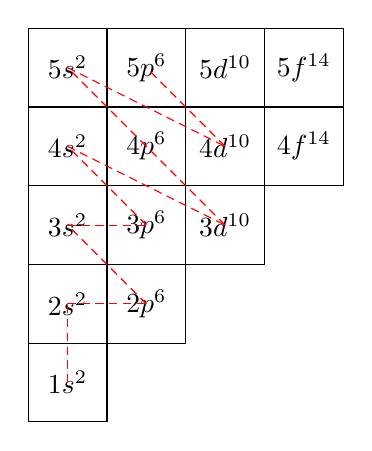
\begin{tikzpicture}
	\draw (0,0) +(-.5,-.5) rectangle ++(.5,.5);
	\draw (0,0) node{$1s^2$};
	\draw (0,1) +(-.5,-.5) rectangle ++(.5,.5);
	\draw (0,1) node{$2s^2$};
	\draw (0,2) +(-.5,-.5) rectangle ++(.5,.5);
	\draw (0,2) node{$3s^2$};
	\draw (0,3) +(-.5,-.5) rectangle ++(.5,.5);
	\draw (0,3) node{$4s^2$};
	\draw (0,4) +(-.5,-.5) rectangle ++(.5,.5);
	\draw (0,4) node{$5s^2$};

	\draw (1,1) +(-.5,-.5) rectangle ++(.5,.5);
	\draw (1,1) node{$2p^6$};
	\draw (1,2) +(-.5,-.5) rectangle ++(.5,.5);
	\draw (1,2) node{$3p^6$};
	\draw (1,3) +(-.5,-.5) rectangle ++(.5,.5);
	\draw (1,3) node{$4p^6$};
	\draw (1,4) +(-.5,-.5) rectangle ++(.5,.5);
	\draw (1,4) node{$5p^6$};

	\draw (2,2) +(-.5,-.5) rectangle ++(.5,.5);
	\draw (2,2) node{$3d^{10}$};
	\draw (2,3) +(-.5,-.5) rectangle ++(.5,.5);
	\draw (2,3) node{$4d^{10}$};
	\draw (2,4) +(-.5,-.5) rectangle ++(.5,.5);
	\draw (2,4) node{$5d^{10}$};

	\draw (3,3) +(-.5,-.5) rectangle ++(.5,.5);
	\draw (3,3) node{$4f^{14}$};
	\draw (3,4) +(-.5,-.5) rectangle ++(.5,.5);
	\draw (3,4) node{$5f^{14}$};

	\draw [draw = red, densely dashed] (0,0) -- (0,1);
	\draw [draw = red, densely dashed] (0,1) -- (1,1);
	\draw [draw = red, densely dashed] (1,1) -- (0,2);
	\draw [draw = red, densely dashed] (0,2) -- (1,2);
	\draw [draw = red, densely dashed] (1,2) -- (0,3);
	\draw [draw = red, densely dashed] (0,3) -- (2,2);
	\draw [draw = red, densely dashed] (2,2) -- (1,3);
	\draw [draw = red, densely dashed] (1,3) -- (0,4);
	\draw [draw = red, densely dashed] (0,4) -- (2,3);
	\draw [draw = red, densely dashed] (2,3) -- (1,4);
	\end{tikzpicture}
	\caption{Auffüllung der Grundzustände}
	\end{figure}
	\\ \newline
	Pro Unterzustand hat man $ N_e = 2(2l+1) $ Elektronen. 
	Die Gesamtzahl der Elektronen in der n-ten Schale entspricht somit $ N_e = 2 \sum_{l}^{n-1} 2l+1 =   2n^2 $

Innerhalb einer Unterschale gelten für die Grundzustände die hierarchischen \textbf{Hund'schen Regeln}: 
\begin{enumerate}
\item Der Gesamtspin  $ S := \lvert \sum_{i} m_{s,i} \rvert $  wird maximal.
\item Der Gesamtdrehimpuls $ L:=  \lvert \sum_{i} m_{l,i} \rvert $ wird maximal.
\item Ist die Unterschale bis zu (einschließlich) halb voll, so wird J minimal d.h \\  $ J := \lvert M_L + M_S \rvert \stackrel{!}{=} \lvert L-S \rvert $ , bei mehr als halb vollen Unterschalden muss $ J \stackrel{!}{=} L+S $ sein. 
\end{enumerate} 

Diese Regeln bestimmen die Feinstruktur des Elements. Regt man das Element an, so gelten diese Regeln nicht mehr.  \newpage Die Schalen-/Orbitalübergänge werden von den sog. \textbf{Auswahlregeln} beherrscht, die wohlgemerkt nicht hierarchisch sind. 
\begin{enumerate}
\item $ \Delta L \  \in $ \{-1,1\}  bei L-S-Kopplung
\item $ \Delta M_L \   \in  $ \{-1,0,1\}  
\item $ \Delta S =0 $ für leichte Atome
\item $\Delta J \  \in $  \{-1,0,1\}   wobei $ \ J =0 \  \rightarrow J=0 \  \textbf{verboten} $
\end{enumerate}

\section{Vielelektronenprobleme} 
Für Elemente mit mehr als einem Elektron gibt es keine analytische Lösung der Schrödinger-Gleichung, auch numerische Verfahren sind mit zunehmender Elektronenzahl extrem aufwändig. Wir machen deshalb folgende Näherungen:
\textbf{Alkaliatome (1.Hauptgruppe)} \newline 
\begin{itemize}
\item Alkaliatome haben nur ein Elektron außerhalb geschlossener Schalen. Die Grundzustände sind immer $ \ ^{2}S_{\frac{1}{2}} $ ( $ n  \in \{2,3,4,...\} $ nicht notiert).
\item Wir betrachten zu Näherung ein \textbf{effektives Potential} $ V_{eff}(r) $ \newline \newline
 $ V_{eff}(r) = - \frac{e^2 Z_{eff}(r)}{r} $ mit $ 1 < Z_{eff}(r) < Z $ \  und  $ Z_ {eff} \stackrel{r\rightarrow \infty}{\rightarrow} 1, \ Z_{eff} \stackrel{r \rightarrow 0}{\rightarrow} Z $
 
\begin{figure}[h]
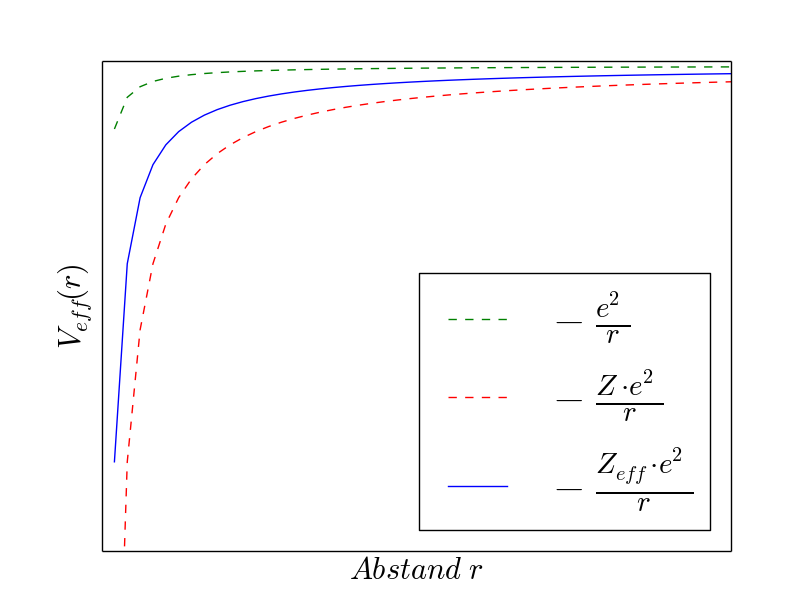
\includegraphics[height= 6cm, width=9cm]{effpot.png}
\caption{ Effektives Potential }
\end{figure}
 \item Dies hebt die $ E_n $ -Entartung bezüglich Z bereits auf (Feinstruktur): \newline
$ E_n(s) < E_n(p) < E_n(d) < E_n(f)$ (für kleine n am stärksten)
\item Für große n und r (wasserstoffähnlich) lässt sich dies so schreiben: 
 	\begin{equation}
 	E_{n,l} = -E_0 \frac{Z_{eff}^2}{n^2} = - \frac{E_0}{n_{eff}^2} = - \frac{E_0}{(n-\delta_{n,l})^2} 			\qquad E_0 = 13.6 \  eV 
 	\end{equation}
 wobei $\delta_{n,l} $ der sog. \textbf{Quantendefekt} ist: $ \delta_{n,l} = n - \sqrt{\frac{E_0}{-E_{n,l}}} \newline  E_{n,l} <\  0  $ ist die real gemessene Energie. 

\end{itemize}
Um allgemeine Vielelektronenprobleme zu lösen, können wir (zumindest bis jetzt) nur nähern indem wir zur Lösung eines Elektron die anderen Elektronen unabhängig voneinander gelöst habe und das entstehen $ V_{eff}(r) $ \textbf{kugelsymmetrisch} ist. \newline
Wir suchen deshalb eine  \textbf{Gesamtwellenfunktion für N Teilchen}. \newline
Diese muss antisymmetrische unter Vertauschung sein, wir nehmen zusätzlich an, dass sie sich als Produkt der Einteilchenwellenfunktionen schreiben lässt. \newline 
Analog zu $ \psi_{ges}(1,2) = \psi_1(1) \psi_2(2) - \psi_2(1) \psi_1(2) $  definieren wir die \\ \textbf{Slaterdeterminante}: 
	\begin{equation}
	  \psi_{ges}(r_1,...,r_N) \ = \  \frac{1}{\sqrt{N!}} \  det \begin{pmatrix} \psi_1(1) & \psi_1(2) & \dots & \psi_1(N) \\ \vdots & \vdots & \vdots & \vdots \\  \psi_N(1) & \psi_N(2) & \dots & \psi_N(N)  \end{pmatrix} 
	\end{equation}
Diese ist total antisymmetrisch unter Spaltenvertauschung als Summe aus N! Produkten. 
\section{Moseley-Gesetz}
Für Eletronen-übergänge zwischen Zuständen wurde empirisch festgestellt, dass $ \sqrt{f} \propto Z $ ist, wobei f die Frequenz des emittiereten Lichts ist. 
\begin{align*}
\textbf{Moseley Gesetz:} \ f \ &= \ E_0 c (\nicefrac{1}{n_2^2} - \nicefrac{1}{n_1^2}) \ (Z-b)^2 \\ 
mit \  c \  = \    \lambda f \ :   \	\lambda \ & = \ E_0 (\nicefrac{1}{n_2^2} - \nicefrac{1}{n_1^2}) \ (Z-b)^2
\end{align*}
für Übergänge $ n_1 \rightarrow n_2 $ , b - Abschirmkonstante \newline
Für das Wasserstoffatom entspricht das Moseley-Gesetz der Rydberg-Formel. \newline
Für wasserstoffähnliche Atome (b=1) gilt : \quad K-Linie: $ n_2 = 1, \  \alpha :  n_1 = 2, \  \beta: n_1 = 3 $ \newline
Für schwere Atome ($ Z > 40 $  )  gilt :  \qquad L-Linie: $ n_2 = 2 , b \approx 7.4 , \ \alpha : \ n_1= 3 , \  \beta: n_1 = 4 $ \newline
Die Auswahlregeln müssen gelten. 

\section{LS-Kopplung,JJ-Kopplung}
....


\chapter{Werkzeuge der Kern- und Teilchenphysik} 

\section{Zerfallsgesetz}
Es gibt 3 verschiedene Zerfallsarten des Radioaktiven Zerfalls.  (A: Nukleonenanzahl , Z: Kernladungszahl)
\begin{itemize}
\item  $ \alpha $  - Zerfall:  $ ^{A}_{Z}X \rightarrow ^{A-4}_{Z-2}Y \ + \ ^{4}_{2}He $  \quad   \\ $ \alpha $ -Strahlung wird mittlels Heliumkernen vermittelt (positiv geladen). 
\item $ \beta $ - Zerfall: 
	\begin{enumerate} 
	\item $ \beta^{-} $ - Zerfall: $ ^{A}_{Z} X\rightarrow ^{A}_{Z+1} Y\ + \ e^{-} \ +\overline{\nu_{e}} $  \\ Beim  $ \beta^{-} $ -Zerfall wird im Kern ein Neutron in ein Proton umgewandelt. Dabei werden eine Elektron und ein Elektron-Antineutrino emittiert.
	\item $ \beta^{-} $ - Zerfall: $ ^{A}_{Z}X \rightarrow ^{A}_{Z-1}Y \ + \ e^{+} \ +\nu_{e} $ \\ Beim $ \beta^{-} $ -Zerfall wird im Kern ein Proton in ein Neutron umgewandelt. Dabei werden eine Elektron und ein Elektron-Neutrino emittiert.
	\end{enumerate}
\item $ \gamma $ -Zerfall :  $ ^{A}_{Z}X^{*} \rightarrow ^{A}_{Z}X + \gamma $ \newline Falls nach einem $ \alpha $ - Zerfall oder $ \beta $ - Zerfall ein Atomkern in einem angeregten Zustand vorliegt, ist $ \gamma $ - Zerfall möglich. Beim Übergang in einen energetisch günstigeren Zustand wird hochfrequente elektromagnetische Strahlung emittiert. Meist folgt der  $ \gamma $ -Zerfall unmittelbar auf einen $ \alpha $ - oder $ \beta $ - Zerfall. \\ 
\newline 
Für die Zerfallsrate(Aktivität) $ A = \frac{d}{dt} N(t)$  gilt die folgende Differentialgleichung: 
\begin{equation}
\frac{d}{dt} N(t) = - \lambda N(t) 
\end{equation}
$ \lambda $ : Zerfallskonstante beschreibt Wahrscheinlichkeit für eine bestimmte radioaktive Zerfallsart. Sie ist unabhängig von Ort und Zeit, aber charakteristisch für den Kern. \newline
Die Lösung dieser Gleichung gibt die Anzahl N der Atome zum Zeitpunkt t an: 
\begin{equation}
N(t) = N_{0} e^{-\lambda \cdot t}
\end{equation}  \newpage
Wobei man in diesem Zusammenhang noch folgende nützliche Größen definiert: 
\begin{itemize}
\item Mittlere Lebensdauer: $ \tau = \nicefrac{1}{\lambda} $ \newline 
Nach dieser Zeit sind nurnoch $\nicefrac{1}{e} $ ($ \approx 37 \% $) der ursprünlichen Atome vorhanden.
\item Halbwertszeit : $ T_{\nicefrac{1}{2}} = \frac{ln(2)}{\lambda} $
Nach dieser Zeit sind nurnoch 50 \% der ursprünlichen Atome vorhanden.
\end{itemize}
\end{itemize}
Der radioaktive Zerfall ist ein stat. Prozess. Die Wahrscheinlichkeit einen zerfallenden Kern anzutreffen ist bei t=0 am größten, danach fällt sie exponentiell ab. 
Diese Wahrscheinlichkeit ist prinzipiell eine Binomial-Verteilung. Für eine hohe Anzahl an Versuchen und eine kleine Wahrscheinlichkeit konvergiert die Binomialverteilung gegen eine Poisson-Verteilung. Diese Näherung lässt sich auf den radioaktiven Zerfall anwenden, da man in der Regel viele Atome (N $\approx 10^{23} $) betrachtet, also eine hohe Anzahl Versuche durchführt, und die Zerfallswahrscheinlichkeit in der Regel klein ist: 
\begin{equation}
p(t) = 1 - e^{-\lambda \cdot t} 
\end{equation}
Somit lässt sich der Zerfall also durch eine Poisson-Verteilung beschreiben mit dem Mittelwert $ \mu = n\cdot p $ und der Standardabweichung  $ \sigma = \sqrt{\mu} $ wobei der Zerfall k-mal eintreten soll. 
\begin{equation}
P(k) = \frac{\mu^k \cdot e^{-\mu} } {k!} 
\end{equation}

\section{Fermis Goldene Regel}
Wir wollen eine Vorraussage für die Übergangsrate $ \lambda $ (Übergangswahrscheinlichkeit pro Zeit), mit der ein Anfangszustand unter dem Einfluss einer Störung in einen anderen Zustand übergeht, treffen. Wir nehmen dabei an, dass es sich um ein an sich zeitlich konstantes System handelt, welches durch den Hamilton-Operator $ H_0 $ beschrieben wird, und durch einen Störoperator V, welcher vergleichsweise klein gegenüber  $ H_0 $ ist, gestört wird. Der gesamte Hamiltonoperator lautet also $ H = H_0 + V $ \newline
Wir formulieren Fermis Goldene Regel: 
\begin{equation}
\lambda_{A->E} = \frac{2\pi}{\hslash} \cdot |\braket{\psi_{E} | V |\psi_{A}}|^2 \cdot \rho_{E} = \frac{dP}{dt}
\end{equation}
Die Übergansrate hängt also davon ab wie stark die Störung V den Anfangszustand $ \psi_A $ und den Endzustand $ \psi_E $ koppelt. Außerdem skaliert die Übergangsrate mit der Anzahl der möglichen Übergänge welche durch die Endzustandsdichte $ \rho_{E} $ beschrieben wird. \newpage 

\textbf{Was ist} $\rho(E)$ \textbf{eigentlich ?}
\ \\ \newline
Wir bezeichnen den Phasenraum unseres Systems als den Raum, der durch die Ortskoordinaten \textbf{x} und die dazugehörigen Impulse \textbf{p} aufgespannt wird. In diesem Raum können wir einem Punkt ein Volumen von $ h^3 = (2\pi \hslash)^3 $ zuordnen (Unschärferelation). \newline 

\textbf{1 Dimension}: \newline
Zunächst betrachten wir einen jeweils eindimensionalen Orts-und Impulsraum mit Zuständen $ (x,p) \in  [x,x+L] \times [p_{x},p_{x}+p] $ In diesem Fall kann die Gesamtfläche Lp mit $ N = \frac{Lp}{2\pi \hslash} $ Zuständen gefüllt werden. Für die Zustandsdichte gilt dann: 
\begin{equation}
 \rho(E) = \frac{dN}{dE} = 2 \frac{dN}{dp} \frac{dp}{dE} = \frac{Lp}{2\pi \hslash} \frac{2m}{p} =  \frac{Lp}{2\pi \hslash} \sqrt{\frac{2m}{E}} 
 \end{equation}
 Wobei wir im letzten Schritt auf Kugelkoordinaten transformieren. 
 Der Faktor 2 kommt daher, dass die Zustände (x,p) und (x,-p) bezüglich der Energie entartet sind, denn $ E = E_{kin} = \frac{p^2}{2m} $ \newline
 
 \textbf{3 Dimensionen}: \newline
 Die Anzahl der Gesamtzustände N ist nun
 \begin{equation}
 N = \frac{1}{2 \pi \hslash} \int d\textbf{x}^3 d\textbf{p}^3 = \frac{V}{2 \pi \hslash} \int d\textbf{p}^3 = \frac{V}{2 \pi \hslash} \int p^2 dp \  d\Omega 
 \end{equation}
 Aus der relativistischen Energie-Impuls-Beziehung $ E^2 = (pc)^2 +  (m_pc^2)^2 $ folgern wir $ \frac{d}{dE} = \frac{E}{pc^2} \frac{d}{dp} $ und erhalten damit für die Zustandsdichte für \textbf{1 Teilchen}
 \begin{equation}
\rho(E) = \frac{dN}{dE} = \frac{V}{(2 \pi \hslash)^3}  \frac{E}{pc^2} \frac{d}{dp}  \int p^2 dp \  d\Omega =  \frac{V}{(2 \pi \hslash)^3} \frac{pE}{c^2} \int d\Omega = \frac{VpE}{2 \pi^2 c^2 \hslash^3}
\end{equation}

Für \textbf{2 Teilchen} addieren sich die Impulse im Mittel zu 0, weshalb die Zustandsdichte konstant ist. Jedoch addieren sich die Energien zu $ E = E_1 + E_2 $
\begin{equation}
dE = dE_1 + dE_2 = \frac{p_1c^2}{E1} dp1 + \frac{p_2c^2}{E2} dp2
\end {equation}
Da $ p_1^2 = p_2^2 $ folgt $  p_1 dp_{1} = p_2 dp_{2} $ 
\begin{align*}
\rightarrow  dE &= \frac{E_1 + E_2}{E_1E_2} c^2 p_1 dp_1  \\
\rightarrow  \rho_2 &=   \frac{V}{(2 \pi \hslash)^3} \frac{E_1E_2}{E_1+E_2} p_{1} \int d\Omega_{1}
\end{align*}
\newpage
Wir können dies auf n Teilchen erweitern
\begin{equation}
\rho_{n} = \frac{V^{n-1}}{(2 \pi \hslash)^{3(n-1)}} \frac{d}{dE} \prod_{i=1}^{n-1} \int d^3p_{i} 
\end{equation}

\section{Wirkungsquerschnitt}
Die bisherigen Überlegungen dienten allesamt dazu die Reaktionsrate einer Zustandsänderung zu quantifizieren. Wir nennen nun eine letzte Größe kennen, die ebenfalls diesen Zweck erfüllt.
Der Wirkungsquerschnitt $ \sigma $ gibt die Stärke einer Reaktion an. Um dies zu begreifen betrachten wir einen konstanten Fluss  $\Phi $ von Teilchen, die allesamt der Sorte a zugehören und auf ein Target der Dicke x aus Teilchen der Sorte b geschossen werden.  

\begin{figure}[h]
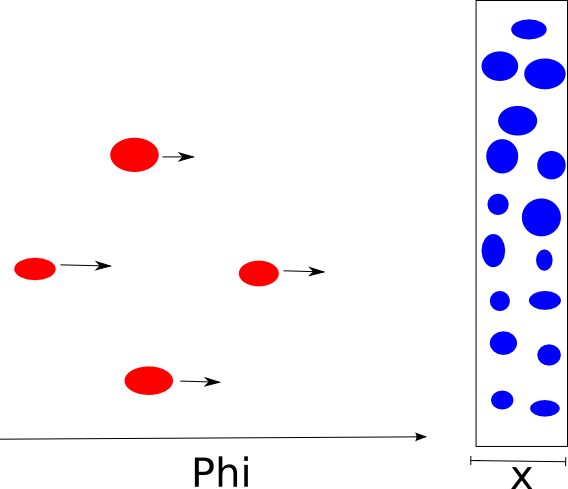
\includegraphics[height= 4cm, width=4cm]{fluss.png}
\caption{Teilchenfluss auf Target}
\end{figure}
Die Reaktionsrate pro Targetteilchen ist $ W = \Phi \cdot \sigma $ 
Die Reaktionsrate im gesamten Target ist $ W \cdot N = \Phi \cdot n_{B} \cdot x $ \\ 
mit N Targetteilchen und der Volumenteilchendichte $ n_B $. \newline

Im Allgemeinen hängt der Wirkungsquerschnitt  $ \sigma $ von der Art der Reaktion ab: 
\begin{itemize}
\item Absorbtion $ \sigma_{A} $
\item elastische Streuung $ \sigma_{E} $
\item inelastische Streuung $ \sigma_{I} $
\end{itemize}
Der Gesamtwirkungsquerschnitt ergibt sich dann via Addition $ \sigma_{Ges} = \sigma_{A} + \sigma_{E} + \sigma_{I}  $ \newline
Für Teilchen die sich innerhalb eines Mediums ausbreiten definiert man die mittlere freie Weglänge $ \lambda = \frac{1}{n_B \sigma}$ \newline
Diese gibt die durchschnittliche Stracke an, die ein Teilchen im Target ohne Wechselwirkun zurücklegen kann. \newpage
Das Volumen in dem 1 Targetteilchen ist ist also $ V = \lambda \cdot \sigma = \nicefrac{1}{n} $  \newline
Anhand der mittleren freien Weglänge lassen sich folgende Größen berechnen: 
\begin{itemize}
\item Anzahl der Strahlteilchen im Targetmaterial : $ N(x) = N_{0} \cdot e^{-\nicefrac{x}{\lambda}} $
\item Kollisionsrate: $ c(x) = - \frac{dN(x)}{dx} = \frac{N_{0}}{\lambda} \cdot e^{-\nicefrac{x}{\lambda}} = c_0 \cdot e^{-\nicefrac{x}{\lambda}} $
\item Wahrscheinlichkeit für Reaktion eines einfallenden Teilchens: $  p(x) = 1- e^{-\nicefrac{x}{\lambda}} $
\end{itemize}
\ \\ 
Aus Dimensionsbetrachtungen lässt sich darauf schliessen, dass der Wirkungsquerschnitt die Dimension einer Fläche hat. Wir werden dies nun veranschaulichen: 
\begin{figure}[h]
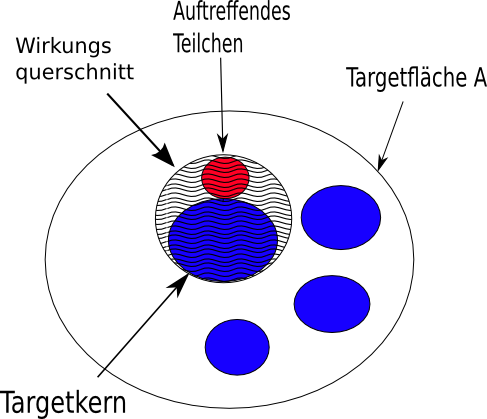
\includegraphics[height=6cm,width=6cm]{wirkungsquerschnitt.png}
\caption{Wirkungsquerschnitt eines Teilchens (rot) das auf ein Targetteilchen (blau) trifft, mit Wirkungsquerschnitt (gewellte Fläche)}
\end{figure} \newline
Im Allgemeinen ist bei Teilchenkollisionen der Wirkungsquerschnitt, die kleinste Fläche, die beide Teilchen komplett einschließt: 
\begin{equation}
\sigma = \pi (r_{K} + r_{P})^2 
\end{equation}
Kernradius: $ r_K $ \qquad Projektilradius: $ r_P $ \newline
Hieraus ergibt sich die Wahrscheinlichkeit, dass das n Projektile mit dem Target wechselwirken, als das Verhältnis der effektiven Flächen:
\begin{equation}
P = \frac{n \sigma}{A}
\end{equation}



\end{document}
 

